\documentclass{beamer}

\usepackage[export]{adjustbox}
\usepackage[many]{tcolorbox}
\usepackage{mathrsfs,amsmath}
\usepackage{tikz}
\usepackage{physics}
\usepackage[ngerman]{babel}

\title{Fourier Transformation}
\subtitle{und ihre Anwendungen}
\author{Elias Kiene, Marek Freunscht}
\date{\today}

\begin{document}

\begin{frame}
    \titlepage
\end{frame}

\begin{frame}
    \frametitle{Themen}
    \begin{enumerate}
        \item Fourier Reihen
        \item Was ist eine Fourier Transformation?
        \item Herleitung der Fourier Transformation
        \item Inverse Fourier Transformation
        \item Herleitung der Diskreten Fourier Transformation
        \item Anwendungen
    \end{enumerate}
\end{frame}

    % !TeX root = ./presentation.tex

\begin{frame}
    \frametitle{Was ist eine Fourier Transformation}
    \begin{itemize}
        \item Approximation eines Signals aus Sinus Frequenzen 
        \item Bildung eines Frequenzspektrums
        \item t-y $\rightarrow$ f-dB
    \end{itemize}    

    \begin{columns}
        \begin{column}{110px}
            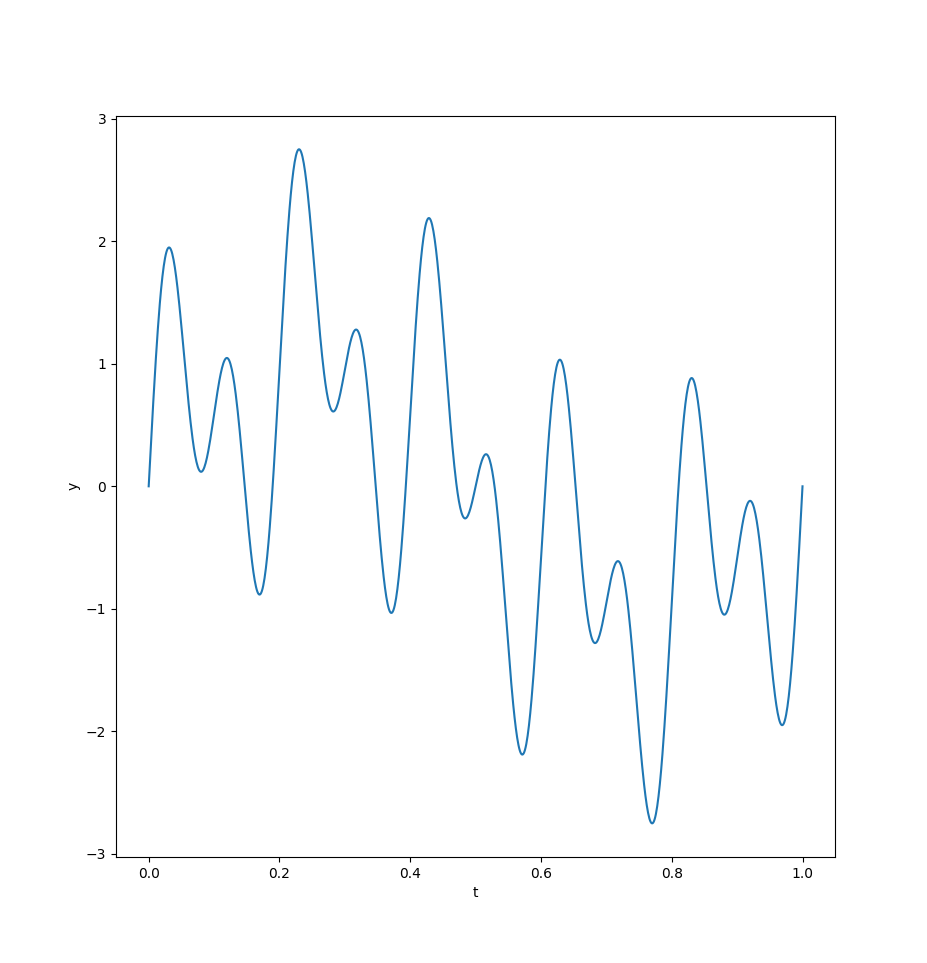
\includegraphics[width=100px]{images/01-what-is-fourier-signal.png}
        \end{column}
        \hspace*{-50px}
        $\rightarrow$
        \begin{column}{60px}
            \centering
            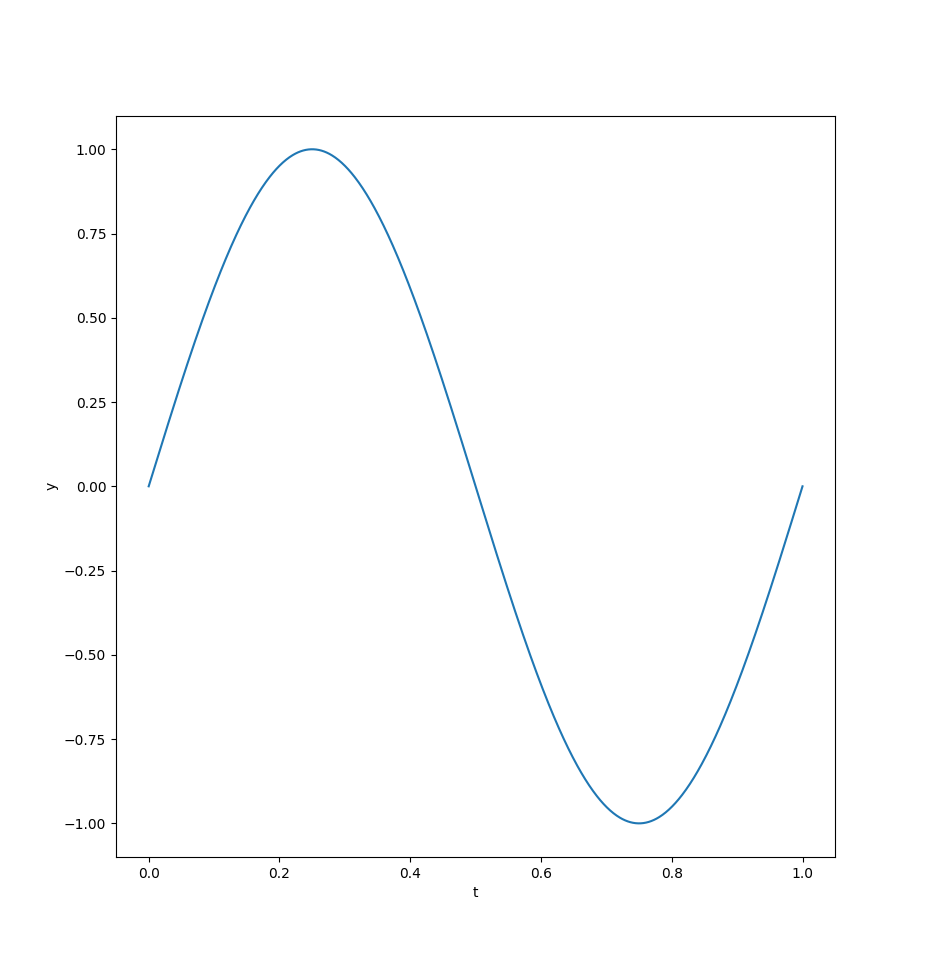
\includegraphics[width=50px]{images/01-what-is-fourier-signal-component-1.png}
            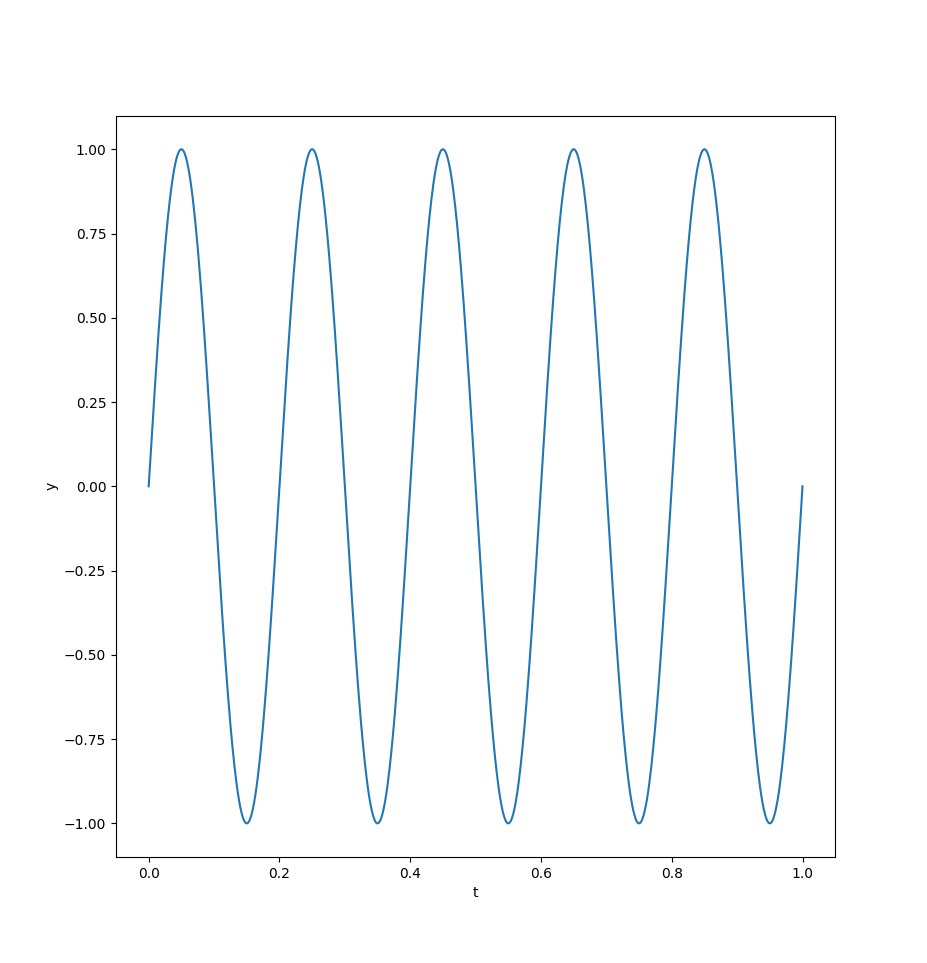
\includegraphics[width=50px]{images/01-what-is-fourier-signal-component-2.png}
            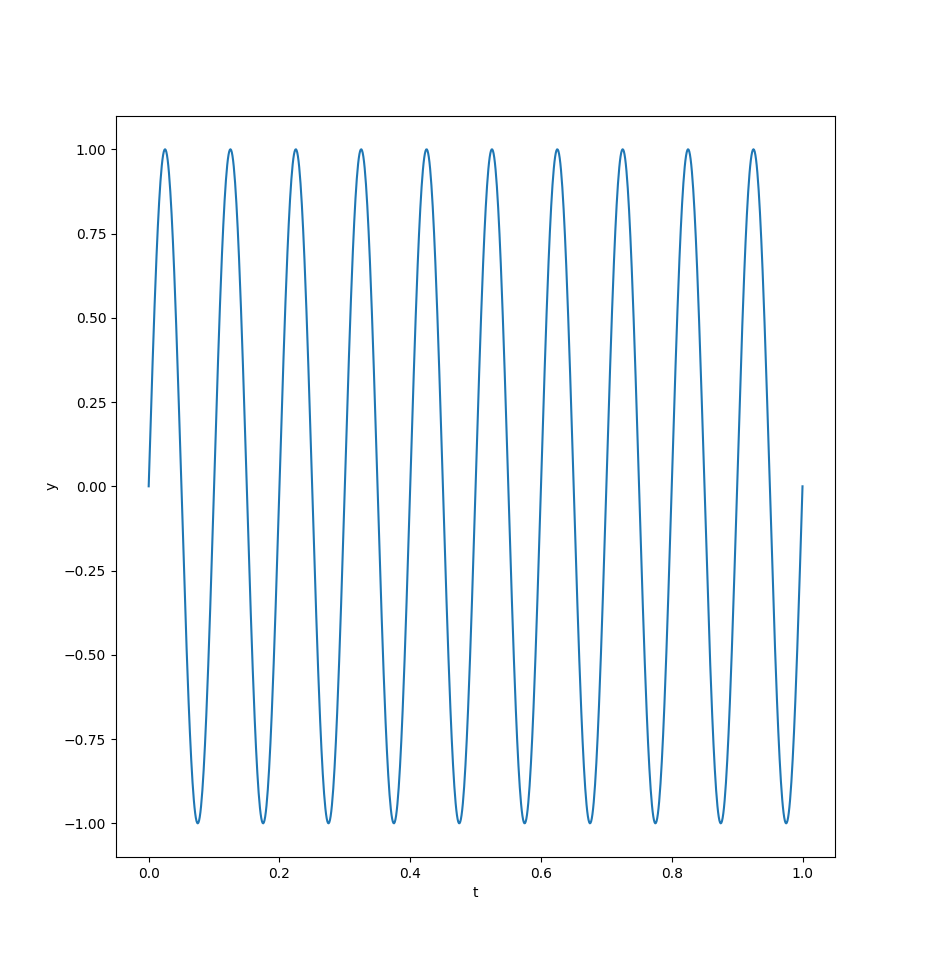
\includegraphics[width=50px]{images/01-what-is-fourier-signal-component-3.png}
        \end{column}
        \hspace*{-40px}
        $\rightarrow$
        \begin{column}{110px}
            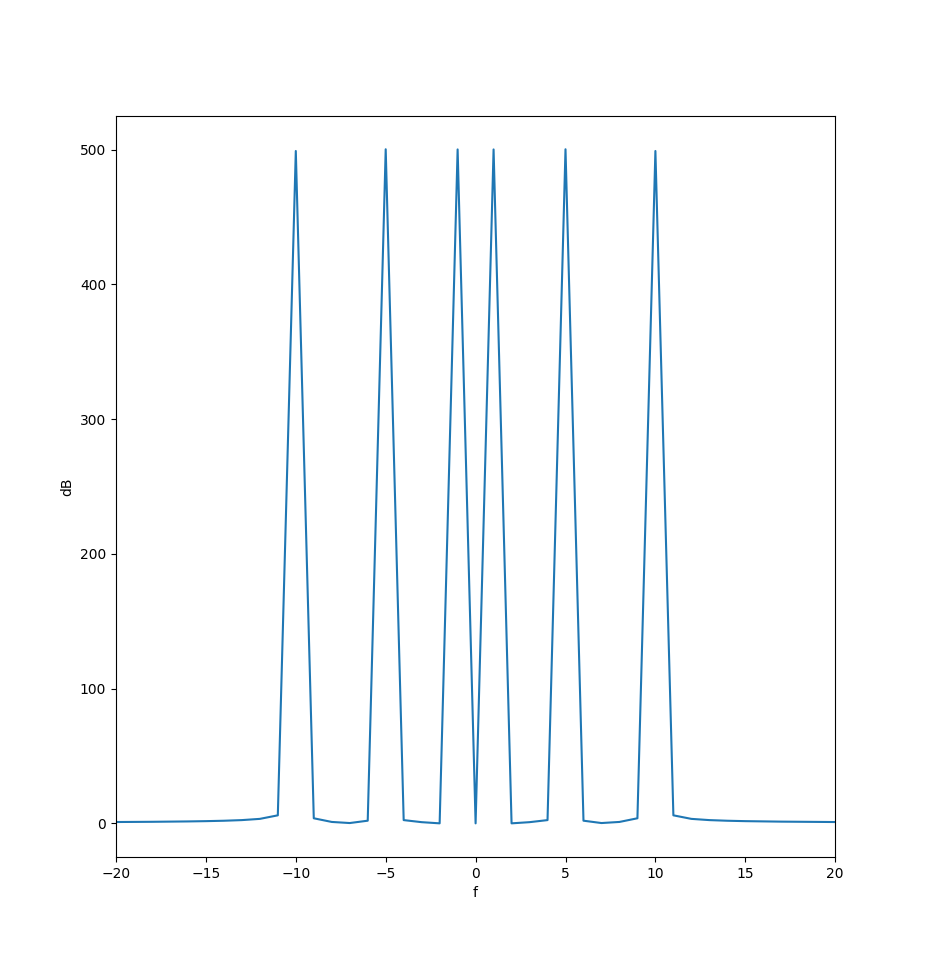
\includegraphics[width=100px]{images/01-what-is-fourier-signal-transform.png}
        \end{column}
    \end{columns}

\end{frame}

    \begin{frame}
    \frametitle{Herleitung der Fourier Transformation} 

    \begin{align*}
        (\mathcal{F} g)(f)=\int_{-\infty}^{\infty}{g(t)\cdot e^{-i2\pi f t}\ dt}
    \end{align*}
\end{frame}

\begin{frame}
    \frametitle{Herleitung der Fourier Transformation}
    \framesubtitle{Eulersche Formel}

    \hspace{-100px}
    \begin{columns}[c]
        \begin{column}{200px}
        \begin{align*}
        e^{i\varphi}=\cos{\varphi}+i\sin{\varphi}
    \end{align*}
\end{column}
\hspace*{-60px}
\begin{column}{100px}
    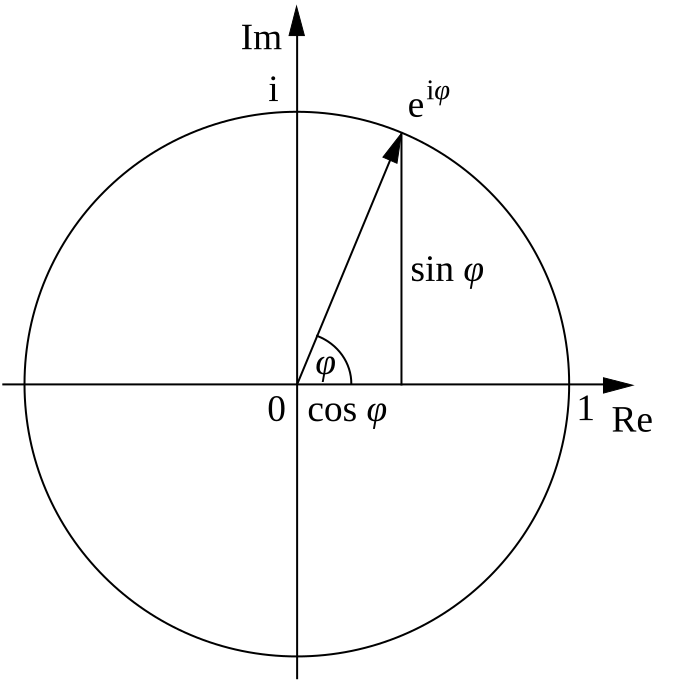
\includegraphics[width=100px]{images/02-deriving-fourier-euler.png}
\end{column}
    \end{columns}
\end{frame}

\begin{frame}
    \frametitle{Herleitung der Fourier Transformation}
    \framesubtitle{Eulersche Formel}

    \hspace{-100px}
    \begin{columns}[c]
        \begin{column}{200px}
        \begin{align*}
        e^{i\varphi}=\cos{\varphi}+i\sin{\varphi}
    \end{align*}
\end{column}
\hspace*{-60px}
\begin{column}{100px}
    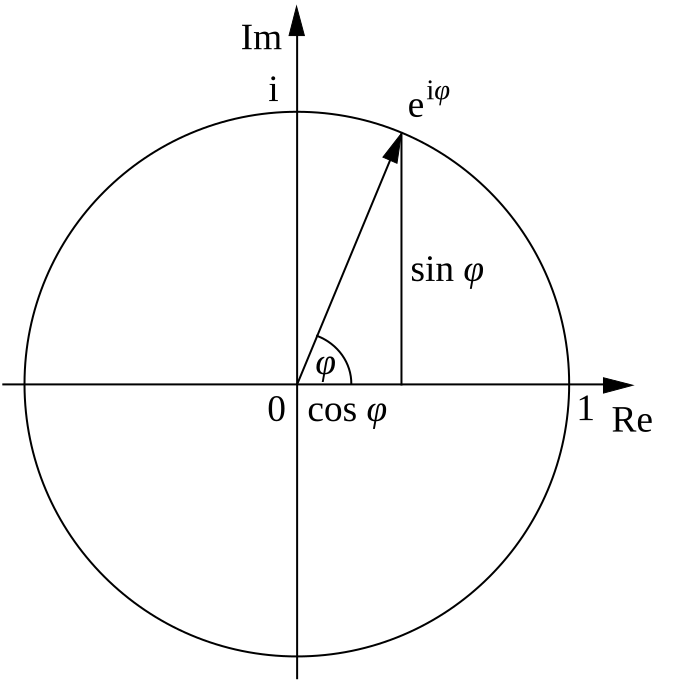
\includegraphics[width=100px]{images/02-deriving-fourier-euler.png}
\end{column}
    \end{columns}
    \vspace{20px}
    Rotieren in der komplexen Ebene mit Frequenz $f$: 
    \begin{align*}
        \varphi&=\omega t=2\pi ft \\
        c(t)&=e^{-i\varphi}\\
            &=e^{-i2\pi f t}
    \end{align*}
\end{frame}

\begin{frame}
    \frametitle{Herleitung der Fourier Transformation}
    \framesubtitle{Rotieren des Signals}

    Signal  $g(t)$ um einen Punkt in der komplexen Ebene rotieren:
    \begin{align*}
        g_c(t, f)=g(t)\cdot e^{-i2\pi f t}
    \end{align*}
    \begin{center}
        \begin{columns}[c]
    \begin{column}{100px}
        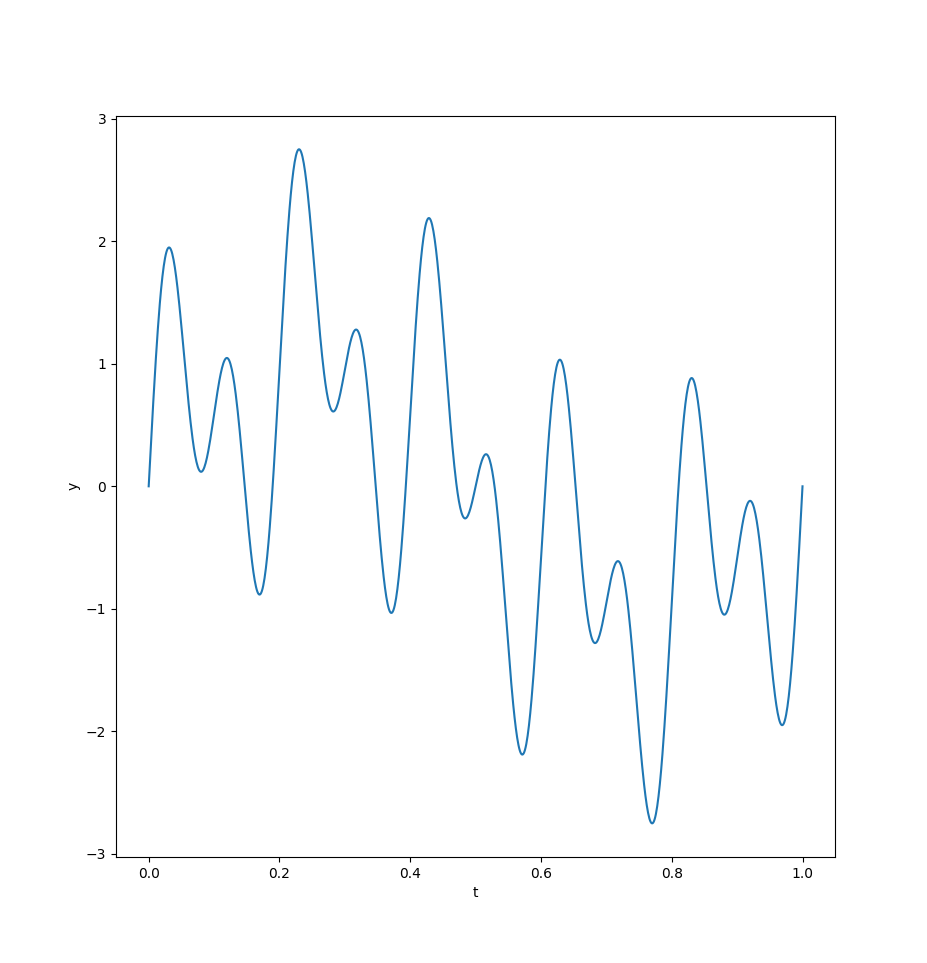
\includegraphics[width=100px]{images/01-what-is-fourier-signal.png}
    \end{column}
    \hspace*{-45px}
    \begin{column}{10px}
        $\overset{\scriptscriptstyle{f=10Hz}}{\parbox{1.1cm}{\rightarrowfill}}$
    \end{column}
    \hspace*{-20px}
    \begin{column}{100px}
        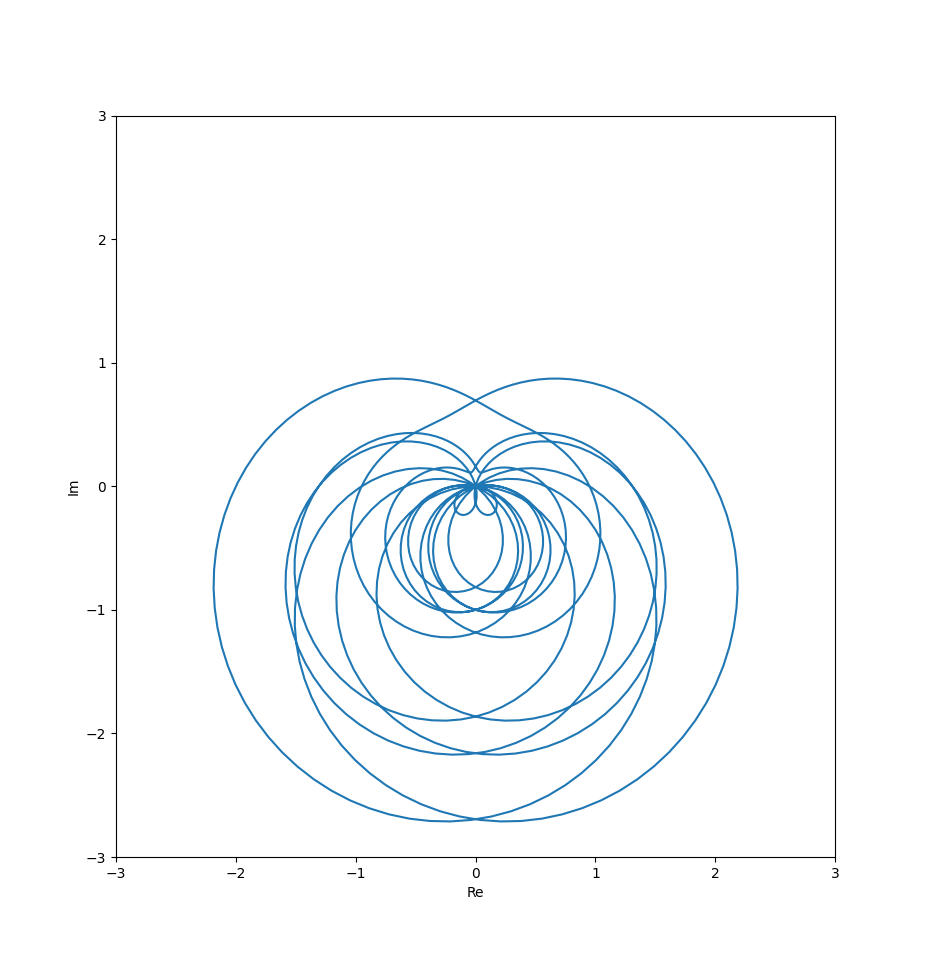
\includegraphics[width=100px]{images/02-deriving-fourier_wrapped_signal.png}
    \end{column}
    \end{columns}
    \end{center}
\end{frame}

\begin{frame}
    \frametitle{Herleitung der Fourier Transformation}
    \framesubtitle{Finden des Durchschnittswertes}
    Durchschnittlichen Wert von $f_c$ finden:
    \begin{align*}
    \frac{1}{N}\cdot \sum_{i=0}^{N}{g(t_i)\cdot e^{-i2\pi f t_i}}
    \end{align*}
    \begin{center}
    $\downarrow$ 
\end{center}
    \begin{align*}
        \frac{1}{t_2-t_1}\cdot \int_{t_1}^{t_2}{g(t)\cdot e^{-i2\pi f t}\ dt}
    \end{align*}
    \begin{itemize}
        \item[?]Entfernen des $\frac{1}{t_2-t_1}$ Terms 
    \end{itemize}
\end{frame}

\begin{frame}
    \frametitle{Herleitung der Fourier Transformation}
    \framesubtitle{Finden des Durchschnittswertes}
    Durchschnittlichen Wert von $f_c$ finden:
    \begin{align*}
        \frac{1}{t_2-t_1}\cdot \int_{t_1}^{t_2}{g(t)\cdot e^{-i2\pi f t}\ dt}
    \end{align*}
    \frametitle{Herleitung der Fourier Transformation}
    Entfernen des $\frac{1}{t_2-t_1}$ Terms:
    \begin{align*}
    \int_{t_1}^{t_2}{g(t)\cdot e^{-i2\pi f t}\ dt}
    \end{align*}
    \begin{itemize}
        \item Wenn eine Frequenz lange im Signal auftaucht, wird der Peak höher
    \end{itemize}
\end{frame}

\begin{frame}
    \frametitle{Herleitung der Fourier Transformation}
    Erweitern der Integrationsgrenzen:
    \begin{align*}
        \int_{-\infty}^{\infty}{g(t)\cdot e^{-i2\pi f t}\ dt}=(\mathcal{F}g)(f)
    \end{align*}

    \vspace{10px}
    \begin{tcolorbox}[colback=red!5!white,colframe=red!75!black,title=Wichtig]
        $(\mathcal{F} g):\mathbb{R}\rightarrow\mathbb{C}$ ist die komplexwertige Fourier Transformation\newline
        $\abs{(\mathcal{F} g)(f)}\ $ beschreibt die Anwesenheit von Frequenz $f$\newline
         $\angle (\mathcal{F} g)(f)\ $ ist die Phasenverschiebung von Frequenz $f$
    \end{tcolorbox}
\end{frame}

    
\begin{frame}
    \frametitle{Inverse Fourier Transformation}
    \begin{columns}
        \begin{column}{80px}
            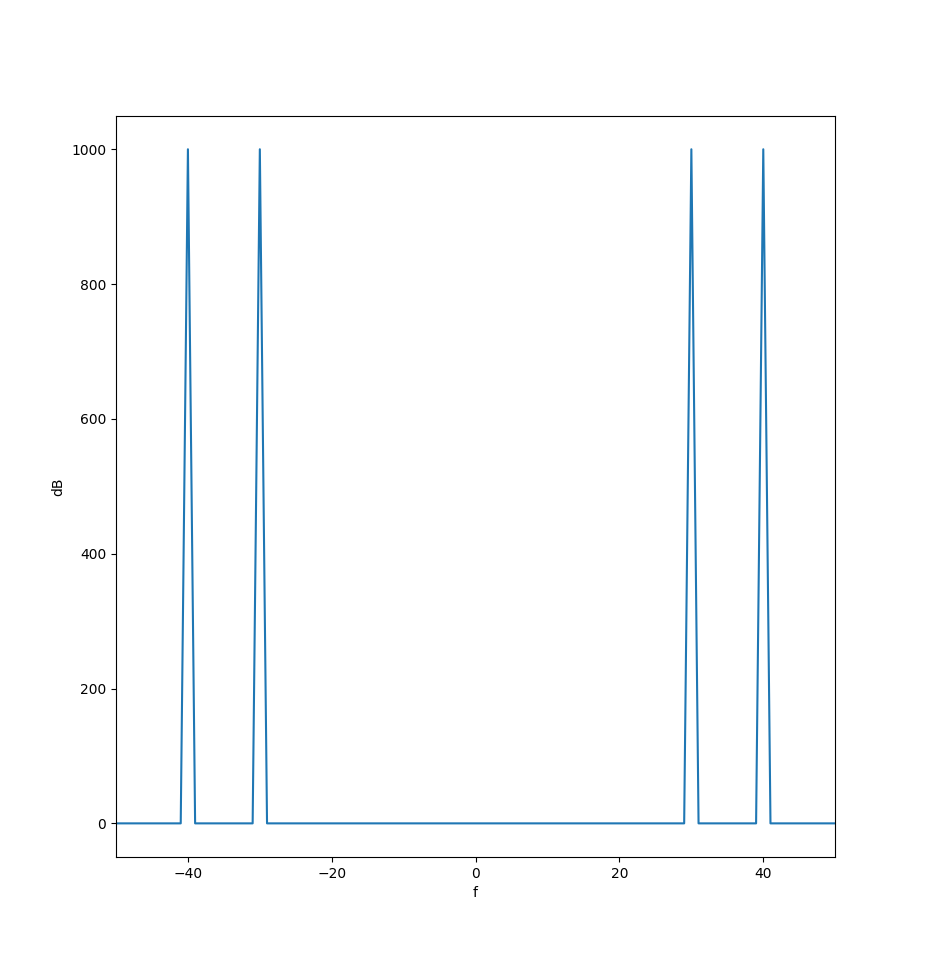
\includegraphics[width=80px, caption=Magnitude]{images/03-ift-mag.png} 
            \centering
            +
            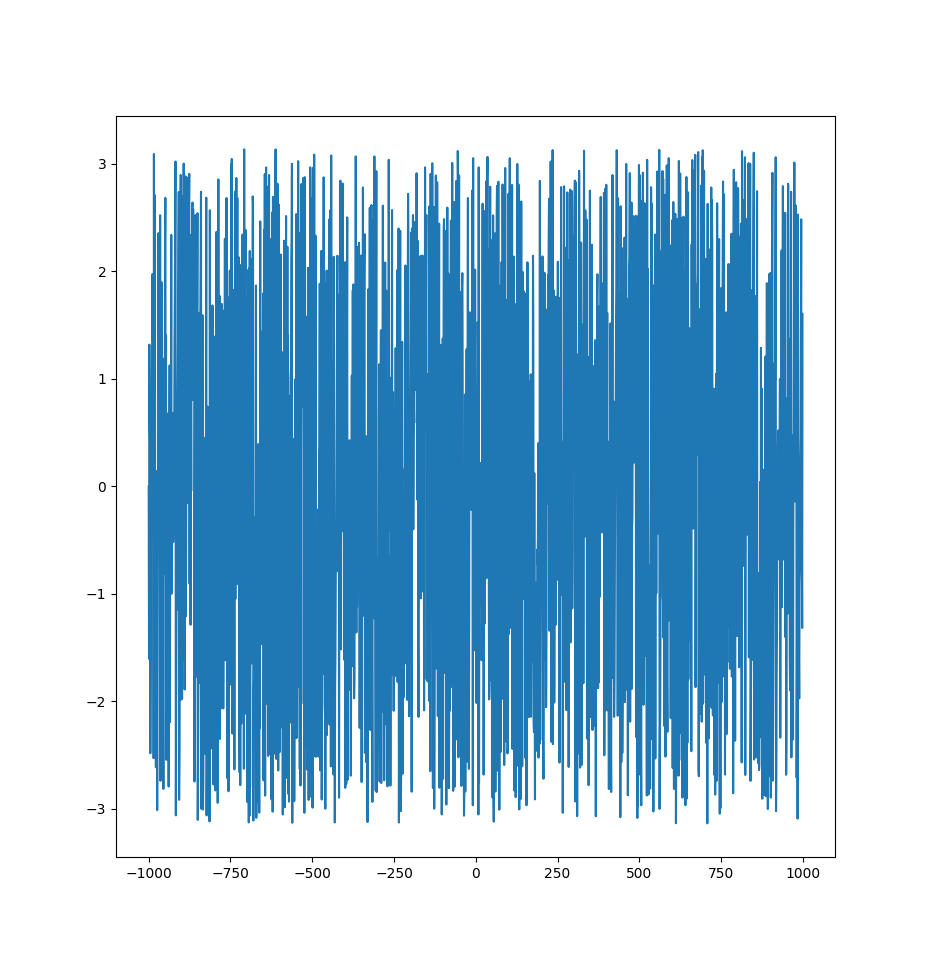
\includegraphics[width=80px]{images/03-ift-phase.png}
        \end{column}
        \hspace*{-40px}
        \begin{column}{5px}
            =
        \end{column}
        \hspace*{-40px}
        \begin{column}{100px}
            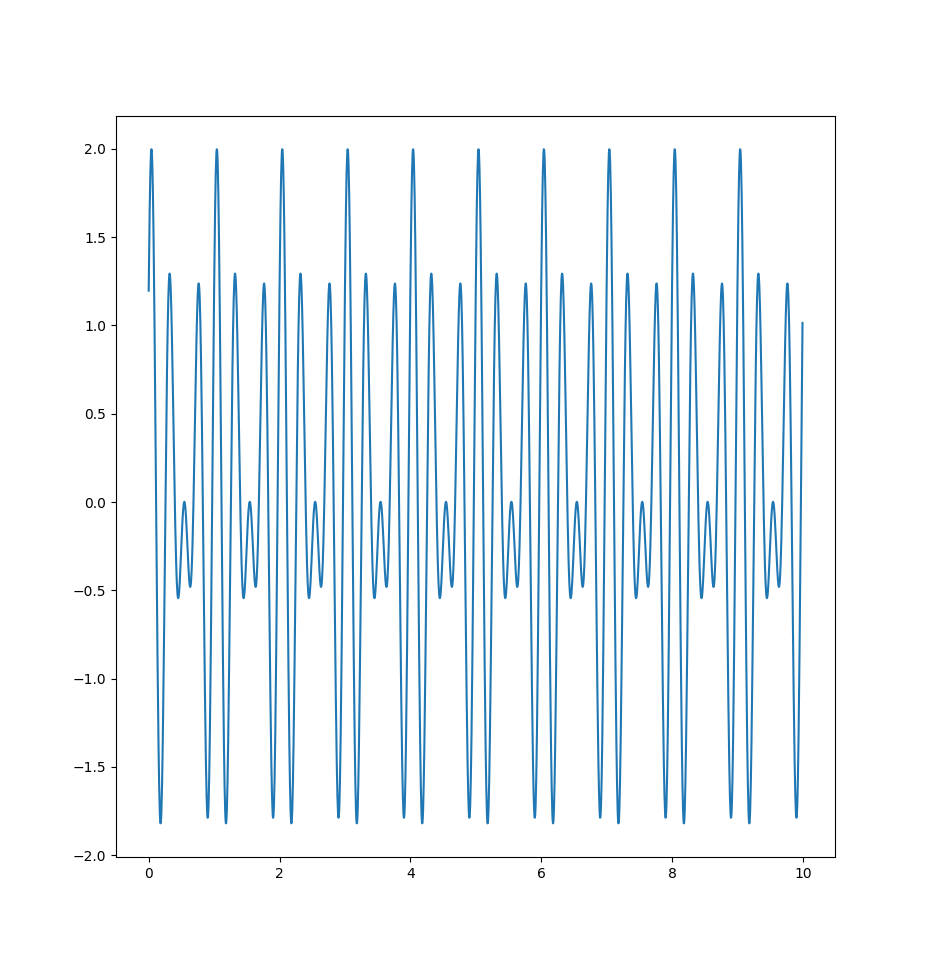
\includegraphics[width=100px]{images/03-ift-reconstructed.png} 
        \end{column}

    \end{columns}
\end{frame}

\begin{frame}
    \frametitle{Inverse Fourier Transformation}
    \begin{align*}
        g(t)=\int_{-\infty}^{\infty}{(\mathcal F g)(f)\cdot  e^{i2\pi f t}\ df}
    \end{align*} 
    \begin{itemize}
        \item Zwischen beiden Transformationen gehen keine Informationen verloren
    \end{itemize}
    \begin{align*}
        \Rightarrow \mathcal{F}^{-1}(\mathcal F g)(f)=g(x)
    \end{align*}
    \vspace*{-15px}
    \begin{itemize}
        \item[?] Wofür wird diese Rücktransformation benutzt
    \end{itemize}
\end{frame}

\begin{frame}
    \frametitle{Inverse Fourier Transformation}
    \begin{align*}
        g(t)=\int_{-\infty}^{\infty}{(\mathcal F g)(f)\cdot  e^{i2\pi f t}\ df}
    \end{align*} 
    \begin{itemize}
        \item Zwischen beiden Transformationen gehen keine Informationen verloren
    \end{itemize}
    \begin{align*}
        \Rightarrow \mathcal{F}^{-1}(\mathcal F g)(f)=g(x)
    \end{align*}
    \vspace*{-15px}
    \begin{itemize}
        \item Besonders nützlich z.B. für das Filtern von Frequenzen
    \end{itemize}
\end{frame}

    
\end{document}

